\section{Results}
\label{sec:results}

\subsection{Primary workflows: preserved contracts, less work}
\label{sec:res-primary}

\begin{table}[t]
  \centering
  \caption{Primary live-provider results ($n=30$ held-out records per family).
  ``Interfaces'' counts provider-visible tool interfaces. All conditions share
  records, model, and grader; \emph{Manual} is hand-written with full workflow
  knowledge (\cref{tab:manual-resources}, \cref{app:stats}).}
  \label{tab:primary}
  \footnotesize
  \setlength{\tabcolsep}{3.5pt}
  \begin{tabular}{@{}lccccccccc@{}}
\toprule
& \multicolumn{3}{c}{Exact held-out contract} & & \multicolumn{5}{c}{Reduction of compiled vs.\ baseline (\%)} \\
\cmidrule(lr){2-4}\cmidrule(lr){6-10}
Family & Base & Compiled & Manual & & Requests & Interfaces & Tokens & Latency & Cost \\
\midrule
Issue-type routing        & 30/30 & \textbf{30/30} & 30/30 & & 50.0 &  0.0 & 39.5 & 51.7 & 32.0 \\
PR-outcome audit          & 30/30 & \textbf{30/30} & 30/30 & & 75.0 & 66.7 & 80.8 & 73.0 & 75.3 \\
Backlog-attention routing & 29/30 & \textbf{30/30} & 30/30 & & 74.8 & 66.3 & 81.4 & 68.9 & 75.1 \\
\midrule
Weighted total ($n=90$)   & 89/90 & \textbf{90/90} & 90/90 & & 66.6 & 44.2 & 63.1 & 64.2 & 58.7 \\
\bottomrule
\end{tabular}

\end{table}

\begin{figure}[t]
  \centering
  \begin{minipage}[t]{0.50\linewidth}
    \centering
    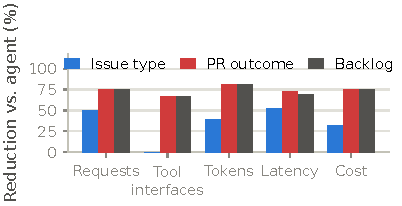
\includegraphics[width=\linewidth]{figures/family_reductions_panel.pdf}
  \end{minipage}\hfill
  \begin{minipage}[t]{0.48\linewidth}
    \centering
    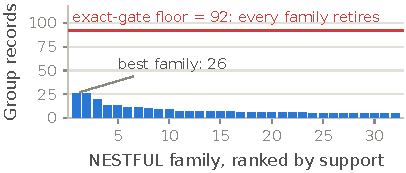
\includegraphics[width=\linewidth]{figures/gate_support_panel.pdf}
  \end{minipage}
  \Description{Left: bar chart of per-family reductions in requests, interfaces,
  tokens, latency, and cost against the unchanged agent. Right: NESTFUL recurring
  families ranked by group-record support, all far below the 92-group exact-gate
  floor.}
  \caption{Left: reduction against the unchanged agent per family (30 held-out
  records each; the values of \cref{tab:primary}). Right: NESTFUL's 32 recurring
  families ranked by group-record support against the 92-group floor of
  \cref{eq:cp}; the best reaches 26, so every family retires
  (\cref{sec:res-refusal}).}
  \label{fig:results}
\end{figure}

Across the 90 held-out records, \method satisfies 90/90 exact contracts and the
unchanged agent 89/90 (\cref{tab:primary}, \cref{fig:results} left), reducing provider requests by
66.6\%, tokens by 63.1\%, latency by 64.2\%, and cost by 58.7\% (per-record
values in \cref{tab:absolute-resources}, \cref{app:stats}); issue-type routing, a
two-read prefix, is the low end of every range in \cref{fig:results}.

The discordant pair is one baseline-only miss (backlog record 5189, an
ungrounded excerpt) against zero compiled-only misses (McNemar $p=1$; one-sided
95\% upper bound on compiled-only discordance 3.3\%, or 2.2\% over 210 records
once the 120-record extension of \cref{app:stats}, which holds one compiled-only
miss, is pooled); a rerun of the same 30 records scored 30/30 in every arm
(\cref{app:limits}), so the miss is stochastic and the result supports
preservation, not superiority or equivalence. Each artifact was
admitted with 92 calibration groups and zero replay-contract violations
($U_{\hat\eta}=0.0498\le0.05$), a bound on the compiled region conditional on
i.i.d.\ groups. The
certificate is compiler-wide for issue-type routing, where one candidate
reached calibration, and per-candidate for PR-outcome and backlog routing,
where two did; correcting for both gives $U=0.0569$, above $\alpha$, so those
two are certified compiler-wide only at $\alpha\ge0.057$ (\cref{cor:frozen},
\cref{tab:multiplicity-accounting} in \cref{app:config}). On \code{gpt-6-luna} and on
Anthropic \code{claude-sonnet-5}, same cohorts, re-discovery from each model's
own traces re-derives two of the three artifacts and refuses the third; the
transfer of the retained artifacts to \code{gpt-6-luna} keeps the structure
with one compiled-only miss in 90 (\cref{app:limits}).

Discovery reaches the manual ceiling: programs written with full workflow
knowledge also reach 90/90 and, on the same axes (\cref{tab:manual-resources}),
tie on requests, issue fewer interfaces, cost marginally less, and lose only on
latency. We claim discovery and admission, not runtime dominance.

\subsection{Time-forward transfer: compile or retire}
\label{sec:res-multirepo}

On the narrower two-read pull-request outcome task across frozen public
repositories (\cref{sec:setup}), \method completes 120/120 exact
contracts on paired held-out records across four of five repositories and retires \code{pytorch/pytorch} at
admission, where no calibration group is accepted at any threshold
(\cref{app:breadth}). The compiled program ran on 80/120
held-out records: every open-class record abstained on the induced verifier's
\code{pr.state} hull (discovery pools held 0--3 open records) and ran the
unchanged agent, so requests fall 44.4\% (66.7\% on dispatched records) and
tokens 52.4\%. A balanced three-repository rerun with all three classes in discovery,
\code{pytorch/pytorch} included, dispatches on 180/180 and reaches 180/180 exact
contracts at 66.7\% fewer requests and 78.4\% fewer tokens
(\cref{tab:multirepo-disaggregated} in \cref{app:breadth}); the refusal was
composition-driven. The hand-written program is more efficient in the core
protocol and tied in the rerun.

\subsection{What binds: sample size, then deployability}
\label{sec:res-refusal}

\begin{table}[t]
  \centering
  \caption{Where refusal happens, and what happens where it does not. Stage
  numbers follow \cref{sec:method} and \cref{fig:pipeline}; ``slots'' is the share of dependency slots with
  a recovered producer, and $n_{\max}$ is the largest family support against the 92
  \cref{eq:cp} requires. ``p/a/w'' is pass/abstain/wrong on each substrate's
  \emph{family-level} replay split, which is held out from a different fit than
  the admission split quoted in the text (\cref{app:external}).}
  \label{tab:funnel}
  \footnotesize
  \setlength{\tabcolsep}{4pt}
  \begin{tabular}{@{}lrrrrrcrc@{}}
\toprule
Substrate & Traces & Slots (1) & Windows (2) & At floor (2) & Synth.\ (4) & Replay p/a/\textbf{w} (5) & $n_{\max}$ (6) & Adm. \\
\midrule
NESTFUL   & 1{,}415 & 96.3\% & 1{,}207 & 32 & 12 & 24 / 12 / \textbf{0} & 26 & \textbf{0} \\
API-Bank  &     212 & 63.5\% &      37 &  8 &  2 &  0 /  2 / \textbf{0} &  8 & \textbf{0} \\
BFCL v4   &     200 & 68.0\% &      86 &  9 &  4 &  3 /  3 / \textbf{0} & 15 & \textbf{0} \\
AppWorld  &     136 & 63.2\% &     136 & 33 &  1 & 34 /  0 / \textbf{0} & \textbf{136} & \textbf{1} \\
\bottomrule
\end{tabular}

\end{table}

The external substrates isolate the binding constraint (\cref{tab:funnel}). All
four pass provenance, synthesis, and replay with \emph{no} wrong execution
(API-Bank's two replay windows abstain rather than pass), but NESTFUL, API-Bank,
and executed BFCL gold plans retire at stage 6 on support alone, $n_{\max}=26$,
$8$, $15<92$, an outcome fixed before the compiler ran. AppWorld's gold solutions reach $n_{\max}=136$, the first external corpus
where \cref{eq:cp} is satisfiable; it admits one artifact at 92/92
zero-violation groups ($U_{\hat\eta}=0.0498$) with 11/11 exact replay on its
sealed split under both pre-registered effect arms, bounded by a step-like gate
and an argument-free program (\cref{app:external}).

Admissibility is not dispatchability: against AppWorld's 28 released baseline
runs (8{,}190 trajectories) the admitted region is eligible at the entry boundary
in $37.9\%$, almost always for full-code agents and almost never for ReAct and
plan-and-execute (\cref{tab:appworld-dispatch} in \cref{app:external}). Those
open by reading API documentation, yet admitting that read as a prologue
recovers only 2 more of 4{,}680, because they rarely execute the region at all
(\cref{app:limits}); the measurement bounds $\varphi$ from above.
